\section{Iterated integrals and hyperlogarithms}

Iterated integrals introduced by Chen~\cite{Chen_IteratedPathIntegrals} possess many appealing combinatorial properties, which will contribute significantly to the construction of $\mathbb H^{\Symb}$ later in Chapter 3. We will review these basic properties. In particular, Proposition~\ref{prop: realization of iterated integrals} states how the evaluation of iterated integrals depends on paths. This proposition is crucial in understanding and computing monodromies of multiple polylogarithms disscussed in Chapter 5.

\subsection{Iterated integrals}

\begin{definition}
Suppose $f_i$ are complex-valued continuous functions on $[a,b]$. The \textit{iterated integral} of $f_1,\cdots,f_n$ is inductively defined by
\begin{equation}
\int_a^bf_1(t)dt\cdots f_n(t)dt=\int_a^b\left(\int_a^tf_1(s)ds\cdots f_{n-1}(s)ds\right)f_n(t)dt
\end{equation}
\end{definition}

\begin{remark}
Note that this is not to be confused with repeated iterated integrals in classical calculus.
\end{remark}

The concept of iterated integrals can be straightforwardly extended to the context of complex manifolds.

\begin{definition}\label{def: iterated integrals}
Suppose $X$ is a complex manifold, and $\omega_i$ are holomorphic one-forms. Let $\gamma$ be a piecewise smooth path on $X$. The \textit{iterated integral} of $\omega_1,\cdots,\omega_n$ along $\gamma$ is defined as
\begin{equation}\label{eq: iterated integral}
\int_\gamma\omega_1\cdots\omega_n=\int\limits_{0\leq t_1\leq\cdots\leq t_n\leq 1}\gamma^*\omega_1(t_1)\wedge\cdots\wedge\gamma^*\omega_n(t_n)
\end{equation}
In particular, we adopt the convention that if $n=0$, the value of the iterated integral is defined to be $1$.
\end{definition}

% $D\subset X$ a simple normal crossing divisor, $\gamma:[0,1]\to X-|D|$ is a piecewise smooth path.

\begin{example}\label{ex: int dlog^n}
One can easily show by induction that
\begin{equation}
\int_a^b\overbrace{\frac{dt}{t}\cdots\frac{dt}{t}}^n=\int_a^b\overbrace{d\log t\cdots d\log t}^n=\dfrac{1}{n!}(\log b-\log a)^n
\end{equation}
% \begin{align*}
% \int_a^b\overbrace{d\log t\cdots d\log t}^n&=\int_a^b\left(\int_a^t\overbrace{d\log t\cdots d\log t}^{n-1}\right)d\log t\\
% &=\int_a^b\dfrac{1}{(n-1)!}(\log t-\log a)^{(n-1)}d\log t\\
% &=\int_a^b\dfrac{1}{(n-1)!}(\log t-\log a)^{(n-1)}d(\log t-\log a)\\
% &=\int_a^b\dfrac{1}{n!}d(\log t-\log a)^n\\
% &=\dfrac{1}{n!}(\log b-\log a)^n
% \end{align*}
\end{example}

\begin{example}
Polylogarithms can be expressed as iterated integrals
\begin{equation}
\int_0^x\frac{dt}{1-t}\overbrace{\frac{dt}{t}\cdots\frac{dt}{t}}^{n-1}=\Li_n(x)
\end{equation}
\end{example}

\begin{proposition}\label{prop: basic properties of iterated integrals}\cite{Hain_TheGeometryOfTheMixedHodgeStructureOnTheFundamentalGroup}
Iterated integrals have the following properties.
\begin{enumerate}[i.]
\item $\displaystyle\int_\gamma\omega_1\cdots\omega_n$ is independent of the parametrization of $\gamma$.
\item Suppose $\gamma^{-1}$ is the opposite path of $\gamma$, then
\begin{equation}
\int_\gamma\omega_1\cdots\omega_n=(-1)^n\int_{\gamma^{-1}}\omega_n\cdots\omega_1
\end{equation}
\item Suppose $\alpha$, $\gamma$ are paths such that $\alpha(1)=\beta(0)$, then
\begin{equation}
\int_{\alpha\beta}\omega_1\cdots\omega_n=\sum_{i=0}^n\int_\alpha\omega_1\cdots\omega_i\int_\beta\omega_{i+1}\cdots\omega_n
\end{equation}
\item Product of iterated integrals satisfies the shuffle product relation
\begin{equation}
\int_\gamma\omega_1\cdots\omega_n\int_\gamma\omega_{n+1}\cdots\omega_{n+m}=\sum_\sigma\int_\gamma\omega_{\sigma(1)}\cdots\omega_{\sigma(n+m)}.
\end{equation}
where $\sigma$ runs over all permutations of $\{1,2,\cdots,n+m\}$ with $\sigma^{-1}(1)<\cdots<\sigma^{-1}(n)$ and $\sigma^{-1}(n+1)<\cdots<\sigma^{-1}(n+m)$
\item $\displaystyle\int_\gamma\omega_1\cdots\omega_n$ only depends on the homotopy class of $\gamma$ in $X$ if $\omega_i$ are closed one forms and $\omega_1\wedge\omega_2=\omega_2\wedge\omega_3=\cdots=\omega_{n-1}\wedge\omega_n=0$ (\cite{Hain_TheGeometryOfTheMixedHodgeStructureOnTheFundamentalGroup}, Proposition 3.1).
\end{enumerate}
\end{proposition}

If we only consider logarithmic differential forms like $d\log(z-a)=\dfrac{dz}{z-a}$, the iterated integral is called a \textit{hyperlogarithm}.

\begin{definition}
Suppose $D$ is a divisor with support $|D|=\bigcup_{i=0}^{n+1}\{a_i\}\subset\mathbb C$, where $a_0\neq a_1$, $a_n\neq a_{n+1}$. Let $\gamma$ be a path from $a_0$ to $a_{n+1}$ that is disjoint from $|D|$ except endpoints, the \textit{hyperlogarithm} $I_\gamma(a_0;a_1,\cdots,a_n;a_{n+1})$ is then defined to be
\begin{equation}\label{eq: itegrated integral def of hyperlog}
\int_\gamma d\log(z-a_1)\cdots d\log(z-a_n)
\end{equation}
\end{definition}

\begin{remark}
Due to Proposition~\ref{prop: basic properties of iterated integrals} (v.), it is easy to see that~\eqref{eq: itegrated integral def of hyperlog} is invariant up to homotopy of $\gamma$ in $\mathbb C-|D|$. We also see by convention that $I_\gamma(a_0;a_{n+1})=1$.
\end{remark}

When the endpoints of $\gamma$ is in $|D|$, we need to justify that~\eqref{eq: itegrated integral def of hyperlog} is still finite, we first prove the following Lemma.

\begin{lemma}\label{lem: power series for hyperlog}\cite{FrancisBrown_SingleValuedHyperlogarithmsAndUnipotentDifferentialEquations}
Suppose $\gamma$ is the straight path from 0 to $z$ and $|z|<\displaystyle\min_{1\leq i\leq d}|a_i|$. Then the iterated integral $I_\gamma(0;a_1,\overbrace{0,\cdots,0}^{n_1-1},\cdots,a_d,\overbrace{0,\cdots,0}^{n_d-1};z)$ has the following power series expansion:
\begin{equation}\label{eq:power series for hyperlog}
\sum_{1\leq m_1<\cdots<m_d}\frac{(-1)^d}{m_1^{n_1}\cdots m_d^{n_d}}\frac{z^{m_d}}{a_1^{m_1}a_2^{m_2-m_1}\cdots a_d^{m_d-m_{d-1}}}
\end{equation}
\end{lemma}

\begin{proof}
First note that $I_\gamma(0;a_1,\overbrace{0,\cdots,0}^{n_1-1},\cdots,a_d,\overbrace{0,\cdots,0}^{n_d-1};z)$ is equal to
\[
\int_0^1\frac{zdt}{tz-a_1}\overbrace{\frac{dt}{t}\cdots\frac{dt}{t}}^{n_1-1}\cdots\frac{zdt}{tz-a_d}\overbrace{\frac{dt}{t}\cdots\frac{dt}{t}}^{n_d-1}
\]
and then we can repeatedly use the fact that
\[
\frac{z}{tz-a}=-\sum_{m\geq1}\frac{z^{m}}{a^{m}}t^{m-1}
\]
\end{proof}

\begin{corollary}
If we replace 0 with $a_0\neq a_1$, and $|z-a_0|<\min\limits_{1\leq i\leq d}|z-a_i|$, \eqref{eq:power series for hyperlog} becomes $I_\gamma(a_0;a_1,\overbrace{a_0,\cdots,a_0}^{n_1-1},\cdots,a_d,\overbrace{a_0,\cdots,a_0}^{n_d-1};z)$ which is equal to
\begin{equation}\label{eq:general power series for hyperlog}
\sum_{1\leq m_1<\cdots<m_d}\frac{(-1)^d}{m_1^{n_1}\cdots m_d^{n_d}}\frac{(z-a_0)^{m_d}}{(a_1-a_0)^{m_1}(a_2-a_0)^{m_2-m_1}\cdots (a_d-a_0)^{m_d-m_{d-1}}}
\end{equation}
\end{corollary}

\vspace{1cm}

Now we can find a piecewise straight path $\gamma'$ homotopic to $\gamma$ that for each segment, the condition for Lemma~\ref{lem: power series for hyperlog} is satisfied. By applying Proposition~\ref{prop: basic properties of iterated integrals} (ii., iii.), we proved that~\eqref{eq: itegrated integral def of hyperlog} is indeed finite.

% With \eqref{eq:general power series for hyperlog}, we can easily derive the derivatives of hyperlogarithms
% \begin{equation}
% \dfrac{d}{dz}I_\gamma(a_0;\cdots,a_d,\overbrace{a_0,\cdots,a_0}^{n_d-1};z)=\begin{cases}
% \dfrac{1}{z-a_d}I_\gamma(a_0;\cdots,a_d,\overbrace{a_0,\cdots,a_0}^{n_d-2};z),\quad n_d>1\\
% \dfrac{1}{z-a_d}I_\gamma(a_0;\cdots,a_{d-1},\overbrace{a_0,\cdots,a_0}^{n_{d-1}-1};z),\quad n_d=1
% \end{cases}
% \end{equation}

The value of $I_\gamma(a_0;a_1,\cdots,a_n;a_{n+1})$ depends on the homotopy class of $\gamma$ and the positions of $a_0,a_1,\cdots,a_{n+1}$, so we think of $I(a_0;a_1,\cdots,a_n;a_{n+1})$ without $\gamma$ as a multi-valued function on
\begin{equation}\label{eq: domain of I(a0;...;a_{n+1})}
\mathcal D_n=\left\{(a_0,\cdots,a_{n+1})\in\mathbb C^{n+2}\middle|a_0\neq a_1,a_n\neq a_{n+1}\right\}
\end{equation}
We would like to show this is actually a holomorphic function. This is a little subtle, so we need to prove the following technical lemma, which is typically ignored by other authors.

\begin{lemma}\label{lem: analytic continuation of I(a0,...,a_{n+1})}
Suppose $(a^0_0,\cdots,a^0_{n+1})\in\mathcal D_n$, and $\gamma_0$ is a piecewise smooth path in $\mathbb C$ with $\gamma_0(0)=a_0^0$, $\gamma_0(1)=a_{n+1}^0$ and disjoint with the rest of distinct $a_i^0$'s, For any $(a_0,\cdots,a_{n+1})$ in some small neighborhood
\[
U_\epsilon=\{|a_0-a^0_0|<\epsilon\}\times\cdots\times\{|a_{n+1}-a^0_{n+1}|<\epsilon\}
\]
of $(a_0^0,\cdots,a_{n+1}^0)$, $I_{\alpha^{-1}\gamma_0\beta}(a_0;a_1,\cdots,a_n;a_{n+1})$ can be written as a power series, where $\alpha$ and $\beta$ are the straight paths from $a_0^0$ to $a_0$ and $a_{n+1}^0$ to $a_{n+1}$ respectively (see Figure~\ref{fig: analytic continuation of iterated integrals}).
\end{lemma}

\begin{proof}
We deploy Proposition~\ref{prop: basic properties of iterated integrals} (iii.)
\begin{multline}
I_{\alpha^{-1}\gamma_0\beta}(a_0;a_1,\cdots,a_n;a_{n+1})=\sum_{0\leq i\leq j\leq n+1}I_{\alpha^{-1}}(a_0;a_1,\cdots,a_i;a_0^0)\\
I_{\gamma_0}(a_0^0;a_{i+1},\cdots,a_j;a_{n+1}^0)I_{\beta}(a_{n+1}^0;a_{j+1},\cdots,a_n;a_{n+1})
\end{multline}

We know that $I_{\gamma_0}(a_0^0;a_{i+1},\cdots,a_j;a_{n+1}^0)$ is holomorphic in $a_{i+1},\cdots,a_j$, and according to Proposition~\ref{prop: basic properties of iterated integrals} (ii.) and Lemma~\ref{lem: power series for hyperlog}
\[
I_{\alpha^{-1}}(a_0;a_1,\cdots,a_i;a_0^0)=(-1)^iI_{\alpha}(a_0^0;a_i,\cdots,a_1;a_0),\qquad I_{\beta}(a_{n+1}^0;a_{j+1},\cdots,a_n;a_{n+1})
\]
can also be written as power series in $a_0,a_1,\cdots,a_i,a_{j+1},\cdots,a_n,a_{n+1}$.
\begin{figure}
\centering
\begin{tikzpicture}[scale=1.5]
\foreach \x/\y/\p/\labelpos/\labeltext in {0/0/a00/below/{$a_0^0$}, -.4/.3/a0/above/{$a_0$}, 2/2/a10/above/{$a_1^0$}, 2/1.5/a1/left/{$a_1$}, 5/1/a20/above/{$a_2^0$}, 5.3/.8/a2/right/{$a_2$}, 4/-1/an0/below/{$a_n^0$}, 3.5/-.7/an/below left/{$a_n$}, 7/-1/anp10/below/{$a_{n+1}^0$}, 8/0/anp1/right/{$a_{n+1}$}}{
    \coordinate (\p) at (\x,\y);
    \draw[fill] (\p) circle (0.03);
    \node at (\p)[\labelpos] {\labeltext};
}
\draw[->-=0.5] (a0) to [curve through={(2,.5)..(4,.5)..(6,0)}] (anp1);
\draw[->-=0.5] (a00) to [curve through={(3,0)}] (anp10);
\draw[->-=0.5, blue, dashed] (a00) to (a0);
\draw[->-=0.5, blue, dashed] (a10) to (a1);
\draw[->-=0.5, blue, dashed] (a20) to (a2);
\draw[->-=0.5, blue, dashed] (an0) to (an);
\draw[->-=0.5, blue, dashed] (anp10) to (anp1);
\node at ($.5*(a00)+.5*(a0)$)[below left] {$\alpha$};
\node at ($.5*(anp10)+.5*(anp1)$)[below right] {$\beta$};
\node at (3,0)[below] {$\gamma_0$};
\node at (4,0.5)[above] {$\gamma_1$};
\end{tikzpicture}
\caption{Analytic continuation of $I(a_0;a_1,\cdots,a_n;a_{n+1})$}
\label{fig: analytic continuation of iterated integrals}
\end{figure}
\end{proof}

\begin{remark}\label{rmk: gamma1 = gamma0 => same integral}
If $\gamma_t$ is a small continuous deformation of $\gamma_0$ such that $|\gamma_t(s)-a^0_i|>\epsilon,\forall a^0_i\notin\{a^0_0,a^0_{n+1}\}$ and $\gamma_1(0)=a_0$, $\gamma_1(1)=a_{n+1}$, then $\gamma_1$ is homotopic to $\alpha^{-1}\gamma_0\beta$ and $I_{\gamma_1}(a_0;a_1,\cdots,a_n;a_{n+1})=I_{\alpha^{-1}\gamma_0\beta}(a_0;a_1,\cdots,a_n;a_{n+1})$.
\end{remark}

\begin{proposition}\label{prop: realization of iterated integrals}
$I(a_0;a_1,\cdots,a_n;a_{n+1})$ defines a multi-valued holomorphic function on $\mathcal D_n$ via analytic continuation. The multi-valuedness comes from different choices of the integration path.
\end{proposition}

\begin{proof}
According to Lemma~\ref{lem: analytic continuation of I(a0,...,a_{n+1})}, $I(a_0;a_1,\cdots,a_n;a_{n+1})$  has distinct local power series expansions depending on the homotopy class of $\gamma$. They define a collection of holomorphic germs $\Gamma$ which is a locally connected subspace of the etale space of $\mathcal O_{\mathcal D_n}$. It is not difficult to see that $\Gamma$ is connected since it is possible to deform between any two integration paths. Therefore, we may think of $I(a_0;a_1,\cdots,a_n;a_{n+1})$ as a maximal analytic continuation of any of its germ (see~\cite{Otto_LecturesOnRiemannSurfaces}, Chapter 1, Section 7).
\end{proof}

\subsection{Regularization}

In this section, we define the iterated integral~\eqref{eq: itegrated integral def of hyperlog} when $a_0=a_1$ or $a_n=a_{n+1}$, where the integral diverges. This process is known as regularization. This is extensively discussed in~\cite{Goncharov_MultiplePolylogarithmsAndMixedTateMotives} and~\cite{FrancisBrown_SingleValuedHyperlogarithmsAndUnipotentDifferentialEquations}. To carry out this process we need to introduce shuffle algebra and Lyndon words.

The non-commutative polynomial algebra $\mathbb Q\langle X_0,X_1,\cdots,X_{d+1}\rangle$ has a shuffle product $\shuffle$ besides product (which is concatenation), defined inductively by $1\shuffle X_i=X_i\shuffle 1=X_i$ and
\begin{multline}
(X_{i_1}X_{i_2}\cdots X_{i_n})\shuffle(X_{j_1}X_{j_2}\cdots X_{j_m})=X_{i_1}(X_{i_2}\cdots X_{i_n}\shuffle X_{j_1}X_{j_2}\cdots X_{j_m})\\
+X_{j_1}(X_{i_1}X_{i_2}\cdots X_{i_n}\shuffle X_{j_2}\cdots X_{j_m})
\end{multline}
Multiplication of iterated integrals (\ref{prop: basic properties of iterated integrals} iii.) also behaves like a shuffle product. In this section, we highlight a way to connect shuffle algebras with hyperlogarithms. First we need to introduce the concept of a Lyndon word. Suppose there is a total order by index on the alphabet, i.e. $X_i\prec X_j$ if $i<j$, then there is the usual lexicographical order on the set of words on $\{X_i\}_{i\in\mathbb N}$.

\begin{definition}
A \textit{Lyndon word} $X_{i_1}\cdots X_{i_n}$ is a word such that
\begin{equation}\label{eq: Lyndon word}
X_{i_1}\cdots X_{i_r}\preceq X_{i_{r+1}}\cdots X_{i_n},\qquad\forall 1\leq r<n
\end{equation}
\end{definition}

\begin{remark}
$\overbrace{X_i\cdots X_i}^{n}$ is a Lyndon word. A Lyndon word consists of more than one letters which ordered as $X_{i_1}\prec\cdots\prec X_{i_n}$ cannot begin with $X_{i_n}$ nor end with $X_{i_1}$.
\end{remark}

\begin{example}
$X_0X_3X_2X_1$ is a Lyndon word, while $X_1X_2X_3X_0$ isn't.
\end{example}

The following fact is well-known and we omit its proof.

\begin{theorem}\cite{Radford_ANaturalRingBasisForTheShuffleAlgebraAndAnApplicationToGroupSchemes}\label{thm:Lyndon words}
$\mathbb Q\langle X_0,\cdots,X_{d+1}\rangle$ forms a commutative ring under $\shuffle$, and the set of Lyndon words form an algebraically independent generating set. In other words, we can express non Lyndon words as Lyndon words in a unique way.
\end{theorem}

\begin{example}\label{ex: Lyndon thm example}
$X_0X_1X_0=(X_0X_1)\shuffle X_0-2X_0^2X_1$
\end{example}

For fixed $a_0,a_{i_1},\cdots,a_{i_m},a_{n+1}$ and a path $\gamma$ from $a_0$ to $a_{n+1}$, we may construct a multiplicative map
\[
\iota_\gamma:\mathbb Q\langle X_0,\cdots,X_{d+1}\rangle\to\mathbb C,\quad X_{i_m}\cdots X_{i_1}\mapsto I_\gamma(a_0;a_{i_1},\cdots,a_{i_m};a_{n+1})
\]
it is clear $\iota_\gamma(w_1\shuffle w_2)=\iota_\gamma(w_1)\iota_\gamma(w_2)$ for any words $w_1,w_2\in\mathbb Q\langle X_0,\cdots,X_{d+1}\rangle$.

Unfortunately, $I_\gamma(a_0;a_{i_1},\cdots,a_{i_m};a_{n+1})$ doesn't make sense in~\eqref{eq: iterated integral} if $a_{i_1}=a_0$ or $a_{i_m}=a_{n+1}$ since the integral then becomes singular at the end points. A workaround is to consider its regularized value.

Consider a piece-wise smooth path from $a_0$ to $a_{n+1}$ with $\gamma'(0)=\lambda$, $\gamma'(1)=\mu$. If we denote $\gamma|_{[\varepsilon,1-\varepsilon]}$ as $\gamma_\varepsilon$ for $\varepsilon>0$ small, we can write $\gamma(\varepsilon)=a_0+\lambda\varepsilon+\varepsilon f(\varepsilon)$, $\gamma(1-\varepsilon)=a_0-\mu\varepsilon+\varepsilon g(\varepsilon)$, for some smooth functions $f,g$ such that $\lim\limits_{\varepsilon\to0}f(\varepsilon)=\lim\limits_{\varepsilon\to0}g(\varepsilon)=0$. Then by Example~\ref{ex: int dlog^n} we have
\begin{multline}
I_{\gamma_\varepsilon}(a_0;\overbrace{a_0,\cdots,a_0}^{m};a_{n+1})=\frac{1}{m!}\left(\log(\gamma(1-\varepsilon)-a_0)-\log(\gamma(\varepsilon)-a_0)\right)^m\\
=\frac{1}{m!}\left(\log(a_{n+1}-a_0-\mu\varepsilon+\varepsilon g(\varepsilon))-\log(\lambda\varepsilon+\varepsilon f(\varepsilon))\right)^m
\end{multline}
\begin{multline}
I_{\gamma_\varepsilon}(a_0;\overbrace{a_{n+1},\cdots,a_{n+1}}^m;a_{n+1})=\frac{1}{m!}\left(\log(\gamma(1-\varepsilon)-a_{n+1})-\log(\gamma(\varepsilon)-a_{n+1})\right)^m\\
=\frac{1}{m!}\left(\log(-\mu\varepsilon+\varepsilon g(\varepsilon))-\log(a_0-a_{n+1}+\lambda\varepsilon+\varepsilon g(\varepsilon))\right)^m
\end{multline}
Or more generally the following proposition

\begin{proposition}\label{prop: I_epsilon = O(log^m(epsilon))}
When $\varepsilon>0$ is small, one has
\[
I_{\gamma_\varepsilon}(a_0;a_{i_1},\cdots,a_{i_m};a_{n+1})=f_0(\varepsilon)+f_1(\varepsilon)\log\varepsilon+\cdots+f_m(\varepsilon)\log^m\varepsilon,
\]
where $f_i$ are analytic around $0$, and $f_0(0)$ is only dependent on the homotopy class of $\gamma$ with fixed $\gamma'(0)$, $\gamma'(1)$.
\end{proposition}

\begin{proof}
If $i_1>0$ and $i_m<n+1$, $f_0(0)=I_{\gamma}(a_0;a_{i_1},\cdots,a_{i_m};a_{n+1})$ will be a regular hyperlogarithm, and $f_1=\cdots=f_m$ will be all be 0. If either $i_1=0$ or $i_m=n+1$, by identifying $I_{\gamma_\varepsilon}(a_0;a_{i_1},\cdots,a_{i_m};a_{n+1})$ as $X_{i_1}\cdots X_{i_m}$ and applying Theorem~\ref{thm:Lyndon words}, we may rewrite $I_{\gamma_\varepsilon}(a_0;a_{i_1},\cdots,a_{i_m};a_{n+1})$ uniquely as products and sums of regular hyperlogarithms and $I_{\gamma_\varepsilon}(a_0;a_0,\cdots,a_0;a_{n+1})$, $I_{\gamma_\varepsilon}(a_0;a_{n+1},\cdots,a_{n+1};a_{n+1})$.
\end{proof}

\begin{definition}
The \textit{regularized value} of $I_\gamma(a_0;a_{i_1},\cdots,a_{i_m};a_{n+1})$ is defined to be $f_0(0)$.
\end{definition}

Therefore, $\iota_\gamma$ is well-defined and multiplicative.

\begin{example}
Suppose $\gamma$ is the straight path from $0$ to $z$. Then the regularized value of $I_\gamma(0;\overbrace{0,\cdots,0}^{n};z)$ is $\dfrac{1}{n!}\log^nz$. The regularized value of $I_\gamma(0;0,a_1,0;z)$ is $I_\gamma(0;a_1,0;z)\log z-2I_\gamma(0;a_1,0,0;z)$, according to Example~\ref{ex: Lyndon thm example}.
\end{example}

\begin{remark}\label{rmk: gamma1 = gamma0 => same reg integral}
Remark~\ref{rmk: gamma1 = gamma0 => same integral} can be generalized for regularized iterated integrals. If either $a_0=a^0_0$, $\gamma_t'(0)=\gamma_0'(0)$ or $a_{n+1}=a^0_{n+1}$, $\gamma_t'(1)=\gamma_0'(1)$, then $\gamma_1$ is homotopic to $\alpha^{-1}\gamma_0\beta$ with fixed $\gamma'(0)$ or $\gamma'(1)$. By Proposition~\ref{prop: I_epsilon = O(log^m(epsilon))},  $I_{\gamma_1}(a_0;a_1,\cdots,a_n;a_{n+1})$, $I_{\alpha^{-1}\gamma_0\beta}(a_0;a_1,\cdots,a_n;a_{n+1})$ have the same regularized values.
\end{remark}

% Combine what we know about Lyndon words and regularization, we have
% \begin{multline}
% \sum_{X_{i_1}\cdots X_{i_m}} I_{\gamma_\varepsilon}(a_0;a_{i_1},\cdots,a_{i_n};a_{n+1})X_{i_1}\cdots X_{i_m}=\exp(\log(\lambda\varepsilon)X_0)\\
% \sum_{X_{i_1}\cdots X_{i_m}} I_{\gamma_\varepsilon}(a_0;a_{i_1},\cdots,a_{i_n};a_{n+1})X_{i_1}\cdots X_{i_m}\exp(\log(-\mu\varepsilon)X_{n+1})
% \end{multline}
% The first sum runs over all words while the second sum only runs over all Lyndon words.

\section{Hopf algebras and Lie coalgebras}

Iterated integrals have the structure of a connected graded Hopf algebra. We review the definition and main properties of a connected graded Hopf algebra. They yield a Lie coalgebra when modded out by non-constant products, which form the theoretic basis for the construction of our model for a motivic complex. We also discuss in detail the symbol map $\Delta_{1,\cdots,1}$, which is useful in generating symbols of multiple polylogarithms. The following discussions can be found in many references, for example~\cite{Radford_HopfAlgebras}.

\subsection{Hopf algebra}

\begin{definition}
Let $k$ be a $\mathbb Z$-algebra. A \textit{$k$-Hopf algebra} $H$ is a $k$-algebra equipped with $k$-algebra homomorphisms
\begin{itemize}
\item a coproduct $\Delta:H\to H\otimes_kH$
\item a counit $\epsilon:H\to k$
\item an antipode $S:H\to H$
\end{itemize}
such that
\begin{itemize}
% \item $m$ is associative: $m(m\otimes1)=m(1\otimes m)$
\item $\Delta$ is coassociative: $(1\otimes\Delta)\Delta=(\Delta\otimes1)\Delta$
% \item $\eta$ is unital: $m(1\otimes\eta)$, $m(1\otimes\eta)$ are the canonical identifications of $k\otimes H\cong H$ and $H\otimes k\cong H$.
\item $\epsilon$ is counital: $(1\otimes\epsilon)\Delta$, $(\epsilon\otimes1)\Delta$ are the canonical isomorphisms $H\otimes k\cong k\otimes H\cong H$
% \item $\Delta,m$ are compatible: $\Delta m=(m\otimes m)(1\otimes\tau\otimes1)(\Delta\otimes\Delta)$, where $\tau(a\otimes b)=b\otimes a$.
% \item $\epsilon,m$ are compatible: $\epsilon m=m(\epsilon\otimes\epsilon)$, where $m(a\otimes b)=ab$.
% \item $\Delta,\eta$ are compatible: $\Delta\eta=(\eta\otimes\eta)\Delta$, where $\Delta(1)=1\otimes1$.
% \item $\eta,\epsilon$ are compatible: $\epsilon\eta=\id_k$.
\item $m(S\otimes1)\Delta=m(1\otimes S)\Delta=\epsilon$, where $m:H\otimes H\to H$ is multiplication
\end{itemize}
\end{definition}

\begin{definition}
A \textit{connected graded Hopf algebra} is a graded $k$-algebra $\bigoplus\limits_{n\geq0} H_n$ that is a Hopf algebra and $\Delta(H_n)\subseteq\bigoplus\limits_{p+q=n}H_p\otimes H_q$, $H_0=k$. We denote the restriction of $\Delta$ to $H_n$ as $\Delta_n=\sum\limits_{p+q=n}\Delta_{p,q}$, where $\Delta_{p,q}:H_n\to H_p\otimes H_q$ are the components.
\end{definition}

\begin{lemma}\label{lem: kernel of counit is H_{>0}}
For any connected graded Hopf algebra $H$, $\ker\epsilon=\bigoplus\limits_{n\geq1}H_n$. If $k$ is a field, then $\ker\epsilon$ is the unique maximal ideal of $H$.
\end{lemma}

\begin{proof}
Suppose $a\in H_p-\ker\epsilon$ is of the smallest degree such that $p>0$. Then by counity we have
\[
a=(\epsilon\otimes 1)\Delta(a)=a+\epsilon(a)
\]
This implies $\epsilon(a)=0$, which is a contradiction. Therefore, $\ker\epsilon=\bigoplus\limits_{n\geq1}H_n$. In the case where $k$ is a field, since $H-\ker\epsilon=k-\{0\}$ are units, so $\ker\epsilon$ is the unique maximal ideal of $H$.
\end{proof}

\begin{lemma}\label{lemma: Delta0,n}
$\Delta_{0,n}(a)=1\otimes a$ and $\Delta_{n,0}(a)=a\otimes 1$
\end{lemma}

\begin{proof}
Suppose $\Delta_{0,n}(a)=\sum c_i\otimes b_i$, since $c_i$ are scalars, this is equal to $1\otimes\left(\sum c_ib_i\right)=1\otimes b$. By Lemma~\ref{lem: kernel of counit is H_{>0}}, $a=(\epsilon\otimes1)\Delta(a)=(\epsilon\otimes1)\Delta_{0,n}(a)=b$. This justifies $\Delta_{0,n}(a)=1\otimes a$. Similar arguments can be made for $\Delta_{n,0}$.
\end{proof}

\begin{definition}
We define the restricted coproduct $\Delta'$ to be $\bigoplus\limits_{\substack{p+q=n\\p>0,q>0}}\Delta_{p,q}$.
\end{definition}

Due to Lemma~\ref{lemma: Delta0,n}, $\Delta'(a)=\Delta(a)-a\otimes1-1\otimes a$. It is not hard to justify that $(1\otimes\Delta')\Delta'=(\Delta'\otimes1)\Delta'$.

\begin{theorem}\label{thm: uniqueness of antipode}
Suppose $H$ is a graded bialgebra (a Hopf algebra without the antipode) with $H_0=k$. There exists a unique antipode map $S$, giving $H$ a Hopf algebra structure.
\end{theorem}

\begin{proof}
First we prove the uniqueness. Suppose $S$ is an antipode, then we have for any $|a|>0$,
\begin{equation}
\begin{aligned}
0&=\epsilon(a)=m(1\otimes S)\Delta(a)\\
&=m(1\otimes S)(1\otimes a + a\otimes 1 + \Delta'(a))\\
&=S(a) + a + m(1\otimes S)\Delta'(a)
\end{aligned}
\end{equation}
This uniquely and inductively defines $S$ as $S(a)=-a-m(1\otimes S)\Delta'(a)$, and in particular, $S(a)=-a$ for $|a|=1$. For the existence of antipodes, we simply define inductively that $S(a)=-a-m(1\otimes S)\Delta'(a)$. We still need to check that $m(1\otimes S)\Delta'=m(S\otimes 1)\Delta'$. Suppose this is true for all $|a|<n$, then for $|a|=n$, assume $\Delta(a)=\sum_ia_{i_1}\otimes a_{i_2}$, we have
\begin{equation}
\begin{aligned}
m(1\otimes S)\Delta'&=m\left(1\otimes\left(-\id-m(1\otimes S)\Delta'\right)\right)\Delta'\\
&=-m\Delta'-\left(1\otimes m(S\otimes 1)\Delta'\right)\Delta'\\
&=-m\Delta'-m(1\otimes S\otimes 1)(1\otimes\Delta')\Delta'\\
&=-m\Delta'-m(1\otimes S\otimes 1)(\Delta'\otimes1)\Delta'\\
&=-m\Delta'-\left(m(1\otimes S)\Delta'\otimes1\right)\Delta'\\
&=m\left(\left(-\id-m(S\otimes 1)\Delta'\right)\otimes1\right)\Delta'\\
&=m(S\otimes 1)\Delta'
\end{aligned}
\end{equation}
\end{proof}

\begin{definition}
We say an ideal $I\subseteq H$ is a Hopf ideal if $\Delta(I)\subseteq I\otimes H+H\otimes I$ and $S(I)\subseteq I$.
\end{definition}

\begin{proposition}\label{prop: quotient Hopf algebra}
If $I\subseteq$ is a Hopf ideal, then the quotient algebra $H/I$ is again a Hopf algebra. If $H$ is graded and $I$ is homogeneous, $H/I$ is also graded.
\end{proposition}

\begin{proof}
Due to the definition of Hopf ideal, the induced coproduct $\Delta$ and induced antipode $S$ are well-defined. So the quotient algebra is a Hopf algebra as well.
\end{proof}

\begin{definition}
Suppose $A$ is an abelian group, consider the tensor algebra $\displaystyle T(A)=\bigoplus_{n=0}^\infty A^{\otimes n}$, endowed with a shuffle product
\begin{equation}
\begin{aligned}
(a\otimes w_1)\shuffle(b\otimes w_2)&=a\otimes (w_1\shuffle(b\otimes w_2))+b\otimes ((a\otimes w_1)\shuffle w_2)\\
\forall a,b\in A&,w_1\in A^{\otimes n},w_2\in A^{\otimes m}
\end{aligned}
\end{equation}
\end{definition}

The following results are well-known, yet their proofs are frequently omitted. We present them here for completeness and future reference.

\begin{proposition}
We can define a graded connected Hopf structure over this shuffle algebra, with restricted coproduct
\begin{equation}
\Delta'(a_1\otimes\cdots\otimes a_n)=\sum_{i=1}^{n-1}\left(a_1\otimes\cdots\otimes a_i\right)\bigotimes\left(a_{i+1}\otimes\cdots\otimes a_n\right)
\end{equation}
and antipode
\begin{equation}
S(a_1\otimes\cdots\otimes a_n)=(-1)^na_n\otimes\cdots\otimes a_1
\end{equation}
\end{proposition}

\begin{proof}
Note that coproduct is defined like deconcatenations of a word. It is trivial to check coassociativity and counity. We are left to check that the antipode satisfies
\begin{equation}\label{eq: induction on S for shuffle algebra}
S(a_1\otimes\cdots\otimes a_n)+a_1\otimes\cdots\otimes a_n+m(1\otimes S)\Delta'(a_1\otimes\cdots\otimes a_n)=0
\end{equation}
If $n=2$, this is trivial, and for $n\geq3$ we see that $m(1\otimes S)\Delta'(a_1\otimes\cdots\otimes a_n)$ equals
\begin{align*}
&\sum_{i=1}^{n-1}(-1)^ia_i\otimes\cdots\otimes a_1\shuffle a_{i+1}\otimes\cdots\otimes a_n\\
&=\sum_{i=1}^{n-1}\Big((-1)^ia_i\otimes\left(a_{i-1}\otimes\cdots\otimes a_1\shuffle a_{i+1}\otimes\cdots\otimes a_n\right)\\
&\qquad+(-1)^ia_{i+1}\otimes\left(a_{i}\otimes\cdots\otimes a_1\shuffle a_{i+2}\otimes\cdots\otimes a_n\right)\Big)\\
&=\sum_{i=1}^{n-1}(-1)^ia_i\otimes\left(a_{i-1}\otimes\cdots\otimes a_1\shuffle a_{i+1}\otimes\cdots\otimes a_n\right)\\
&\quad-\sum_{i=2}^{n}(-1)^{i}a_{i}\otimes\left(a_{i-1}\otimes\cdots\otimes a_1\shuffle a_{i+1}\otimes\cdots\otimes a_n\right)\\
&=-a_1\otimes a_2\otimes\cdots\otimes a_n-(-1)^na_{n}\otimes a_{n-1}\otimes\cdots\otimes a_1
\end{align*}
This proves~\eqref{eq: induction on S for shuffle algebra}.
\end{proof}

\begin{definition}
Due to coassociativity, we can decompose $\Delta^{\circ k}$ into the sum of components of 
\[
\Delta_{n_1,\cdots,n_k}:H_n\to\bigoplus\limits_{\substack{n_1+\cdots+n_k=n\\n_i\geq0}}H_{n_1}\otimes\cdots\otimes H_{n_k}
\]
And we denote
\begin{equation}
\Delta_{n_1,\cdots,n_k}(a)=\sum_{i}a^{(n_1,\cdots,n_k)}_{i1}\otimes\cdots\otimes a^{(n_1,\cdots,n_k)}_{ik}
\end{equation}
We omit $(n_1,\cdots,n_k)$ when the context is clear.
\end{definition}

\begin{definition}
The symbol map $\Delta_{1,\cdots,1}:H\to T^*H_1$ is the direct sum of $\Delta_{1,\cdots,1}:H_n\to T^nH_1$
\end{definition}

\begin{proposition}
% For any graded connected Hopf algebra $H$, the tensor algebra $T^*H_1$ is again naturally a graded connected Hopf algebra with shuffle product and coproduct defined in the above sense. 
$\Delta_{1,\cdots,1}$ is a morphism of graded Hopf algebras.
\end{proposition}

\begin{proof}
To show that $\Delta_{1,\cdots,1}$ preserves product we need
\begin{equation}\label{eq:symbol of product is the shuffle product of symbols}
\Delta_{1,\cdots,1}(ab)=\Delta_{1,\cdots,1}(a)\shuffle\Delta_{1,\cdots,1}(b)
\end{equation}
for any $|a|=k,|b|=l$. Let's assume
\[
\Delta_{1,k-1}(a)=\sum_ia^{(1,k-1)}_{i1}\otimes a^{(1,k-1)}_{i2},\qquad \Delta_{1,l-1}(b)=\sum_jb^{(1,l-1)}_{j1}\otimes b^{(1,l-1)}_{j2}.
\]
Since $\Delta(ab)=\Delta(a)\Delta(b)$, we have
\begin{align*}
\Delta_{1,k+l-1}(ab)&=\Delta_{1,k-1}(a)\Delta_{0,l}(b)+\Delta_{0,k}(a)\Delta_{1,l-1}(b)\\
&=\left(\sum_ia_{i1}\otimes a_{i2}\right)(1\otimes b)+(1\otimes a)\left(\sum_jb_{j1}\otimes b_{j2}\right)\\
&=\sum_ia_{i1}\otimes(a_{i2}b)+\sum_jb_{j1}\otimes(ab_{j2}),
\end{align*}
Note that
\[
\Delta_{1,\cdots,1}(a)=(\id\otimes\Delta_{1,\cdots,1})\circ\Delta_{1,k-1}(a)=\sum_ia_{i1}\otimes\Delta_{1,\cdots,1}(a_{i2}),
\]
similarly
\[
\Delta_{1,\cdots,1}(b)=(\id\otimes\Delta_{1,\cdots,1})\circ\Delta_{1,l-1}(b)=\sum_jb_{j1}\otimes\Delta_{1,\cdots,1}(b_{j2}).
\]
So we have
\begin{align*}
\Delta_{1,\cdots,1}(ab)&=(\id\otimes\Delta_{1,\cdots,1})\circ\Delta_{1,k+l-1}(ab)\\
&=\sum_ia_{i1}\otimes\Delta_{1,\cdots,1}(a_{i2}b)+\sum_jb_{j1}\otimes\Delta_{1,\cdots,1}(ab_{j2})\\
&=\sum_ia_{i1}\otimes(\Delta_{1,\cdots,1}(a_{i2})\shuffle\Delta_{1,\cdots,1}(b))+\sum_jb_{j1}\otimes(\Delta_{1,\cdots,1}(a)\shuffle\Delta_{1,\cdots,1}(b_{j2}))
\end{align*}
The last equality is by induction on lower weight (\eqref{eq:symbol of product is the shuffle product of symbols} is automatic when $k=0$). On the other hand
\begin{align*}
&\Delta_{1,\cdots,1}(a)\shuffle\Delta_{1,\cdots,1}(b)\\
&=\left(\sum_ia_{i1}\otimes\Delta_{1,\cdots,1}(a_{i2})\right)\shuffle\left(\sum_jb_{j1}\otimes\Delta_{1,\cdots,1}(b_{j2})\right)\\
&=\sum_{i,j}a_{i1}\otimes\Delta_{1,\cdots,1}(a_{i2})\shuffle b_{j1}\otimes\Delta_{1,\cdots,1}(b_{j2})\\
&=\sum_{i,j}a_{i1}\otimes(\Delta_{1,\cdots,1}(a_{i2})\shuffle b_{j1}\otimes\Delta_{1,\cdots,1}(b_{j2}))+b_{j1}\otimes(a_{i1}\otimes\Delta_{1,\cdots,1}(a_{i2})\shuffle\Delta_{1,\cdots,1}(b_{j2}))\\
&=\sum_{i}a_{i1}\otimes\left(\Delta_{1,\cdots,1}(a_{i2})\shuffle\sum_jb_{j1}\otimes\Delta_{1,\cdots,1}(b_{j2})\right)\\
&\qquad+\sum_jb_{j1}\otimes\left(\sum_ia_{i1}\otimes\Delta_{1,\cdots,1}(a_{i2})\shuffle\Delta_{1,\cdots,1}(b_{j2})\right)\\
&=\sum_{i}a_{i1}\otimes(\Delta_{1,\cdots,1}(a_{i2})\shuffle\Delta_{1,\cdots,1}(b))+\sum_jb_{j1}\otimes(\Delta_{1,\cdots,1}(a)\shuffle\Delta_{1,\cdots,1}(b_{j2}))
\end{align*}
To show $\Delta_{1,\cdots,1}$ preserves coproduct (to reduce confusion, we use $\bigotimes$ in $T(A)\bigotimes T(A)$) we need
\begin{equation}
(\Delta_{1,\cdots,1}\bigotimes\Delta_{1,\cdots,1})\circ\Delta(a)=\Delta\circ\Delta_{1,\cdots,1}(a)
\end{equation}
First note that for any $|a|=n$
\begin{align*}
\Delta_{1,\cdots,1}(a)&=(\Delta_{1,\cdots,1}\otimes\Delta_{1,\cdots,1})\circ\Delta_{k,n-k}(a)\\
&=\Delta_{1,\cdots,1}\otimes\Delta_{1,\cdots,1}\left(\sum_{i_k}a^{(k,n-k)}_{i_k1}\otimes a^{(k,n-k)}_{i_k2}\right)\\
&=\sum_{i_k}\left(\Delta_{1,\cdots,1}\left(a^{(k,n-k)}_{i_k1}\right)\otimes\Delta_{1,\cdots,1}\left(a^{(k,n-k)}_{i_k2}\right)\right)\\
&=\sum_ja^{(1,\cdots,1)}_{j1}\otimes\cdots\otimes a^{(1,\cdots,1)}_{jn}
\end{align*}
Therefore
\begin{align*}
(\Delta_{1,\cdots,1}\bigotimes\Delta_{1,\cdots,1})\circ\Delta(a)&=\sum_{k=0}^n\sum_{i_k}\Delta_{1,\cdots,1}\left(a^{(k,n-k)}_{i1}\right)\bigotimes\Delta_{1,\cdots,1}\left(a^{(k,n-k)}_{i2}\right)\\
&=\sum_{k=0}^n\sum_ja^{(1,\cdots,1)}_{j1}\otimes\cdots\otimes a^{(1,\cdots,1)}_{jk}\bigotimes a^{(1,\cdots,1)}_{j(k+1)}\otimes\cdots\otimes a^{(1,\cdots,1)}_{jn}\\
&=\sum_j\sum_{k=0}^na^{(1,\cdots,1)}_{j1}\otimes\cdots\otimes a^{(1,\cdots,1)}_{jk}\bigotimes a^{(1,\cdots,1)}_{j(k+1)}\otimes\cdots\otimes a^{(1,\cdots,1)}_{jn}\\
&=\sum_j\Delta\left(a^{(1,\cdots,1)}_{j1}\otimes\cdots\otimes a^{(1,\cdots,1)}_{jn}\right)\\
&=\Delta\left(\sum_ja^{(1,\cdots,1)}_{j1}\otimes\cdots\otimes a^{(1,\cdots,1)}_{jn}\right)\\
&=\Delta\circ\Delta_{1,\cdots,1}(a)
\end{align*}
\end{proof}

\subsection{Lie coalgebra}

The quotient of a Hopf algebra $H$ by products admits the structure of a Lie coalgebra, which is graded if $H$ is connected graded. We now give the formal definition of a Lie coalgebra.

\begin{definition}\label{def: Lie coalgebra}
Let $k$ be a $\mathbb Z$-algebra. A Lie coalgebra $L$ is a module over $k$ with a linear mapping called the \textit{cobracket} $\delta:L\to L\wedge L$, such that $(\delta a)\wedge b=a\wedge(\delta b)$ and $\delta(1\wedge\delta)=\delta(\delta\wedge1)$. $\delta$ can be extend to a linear mapping $\delta:\bigwedge^nL\to\bigwedge^{n+1}L$
\begin{equation}
\delta(a_1\wedge\cdots\wedge a_n)=\sum_{i=1}^n(-1)^{i+1}a_1\wedge\cdots\wedge(\delta a_i)\wedge\cdots\wedge a_n
\end{equation}
This forms a chain complex known as the \textit{Chevalley-Eilenberg complex} $\bigwedge^*L$
\begin{equation}
L\xrightarrow{\delta}L\wedge L\xrightarrow{\delta}L\wedge L\wedge L\xrightarrow{\delta}\cdots
\end{equation}
\end{definition}

\begin{definition}\label{def: graded Lie coalgebra}
We say that a Lie coalgebra $L$ is \textit{graded} if $L=\bigoplus_iL_i$ and $\delta(L_n)\subseteq\bigoplus_{p+q=n}L_p\wedge L_q$. The degree $n$ part of $\bigwedge^* L$ is
\[
L_n\to \bigoplus_{p+q=n}L_p\wedge L_q\to \bigoplus_{p+q+r=n}L_p\wedge L_q\wedge L_r\to\cdots\to L_1^{\wedge n}
\]
denoted as $\left(\bigwedge^* L\right)_n$
\end{definition}

\begin{example}
$\left(\bigwedge^* L\right)_2$ reads
\[
L_2\to\textstyle\bigwedge^2L_1
\]
$\left(\bigwedge^* L\right)_3$ reads
\[
L_3\to L_2\otimes L_1\to\textstyle\bigwedge^3L_1
\]
$\left(\bigwedge^* L\right)_4$ reads
\[
L_4\to L_3\otimes L_1\oplus\textstyle\bigwedge^2L_2\to L_2\oplus\bigwedge^2L_1\to\bigwedge^4L_1
\]
\end{example}

% \begin{corollary}
% If $H$ is a connected graded Hopf algebra, then $H/(H_{>0}\cdot H_{>0})$ is a graded Lie coalgebra.
% \end{corollary}

It is known that there exists a projection map on a connected graded Hopf algebra $H$ over $\mathbb Q$, whose image can be canonically identified with $H$ modulo products.
% This map one-forms of multiple polylogarithms introduced in Chapter 3 factors through this projection map (see Theorem~\ref{thm: one-form map factor through Gangl's projection map P}).

\begin{definition}\label{def: projection map P}\cite{CharltonDuhrGangl_SingleValuedPolylogs}
Suppose $H$ is a connected graded Hopf algebra over a field $\mathbb Q$ and denote $H_{>0}=\bigoplus_{i>0}H_i$. First we define $R:H\to H$ inductively by $R(x)=nx-m(1\otimes R)\Delta'(x)$ where $|x|=n$ and $m$ is multiplication. The projection map $P:H\to H$ is simply such that $P|_{H_n}=\dfrac{1}{n}R_n$.
\end{definition}

\begin{proposition}
$P$ is an idempotent map with $\ker P=H_{>0}\cdot H_{>0}$.
\end{proposition}

\begin{proof}
It is straightforward to check that $\ker P\subseteq H_{>0}\cdot H_{>0}$. Let's prove $H_{>0}\cdot H_{>0}\subseteq\ker P$. Suppose $|x|=k$, $|y|=l$ and $k,l>0$, and write
\[
% \Delta'(x)=\sum_{0<k<n}x^{(k,n-k)}_{i1}\otimes x^{(k,n-k)}_{i2},\qquad \Delta'(y)=\sum_{0<l<m}y^{(l,m-l)}_{j1}\otimes y^{(l,m-l)}_{j2}
\Delta'(x)=\sum_{i}x_{i1}\otimes x_{i2},\qquad \Delta'(y)=\sum_{j}y_{j1}\otimes y_{j2}
\]
Then we have
\[
R(x)=kx-\sum_i x_{i1}R(x_{i2}),\qquad R(y)=ly-\sum_j y_{j1}R(y_{j2})
\]
and
\begin{multline*}
\Delta'(xy)=\sum_{i,j}x_{i1}y_{j1}\otimes x_{i2}y_{j2}+\sum_{i}\left(x_{i1}y\otimes x_{i2}+x_{i1}\otimes x_{i2}y\right)\\
+\sum_j\left(xy_{j1}\otimes y_{j2}+y_{j1}\otimes xy_{j2}\right)+x\otimes y+y\otimes x
\end{multline*}
By induction, we may assume that $R$ annihilates products of lower weights, and we get
\begin{align*}
R(xy)&=(k+l)xy-m(1\otimes R)\Delta'(xy)\\
&=(k+l)xy-\left(\sum_{i}x_{i1}yR(x_{i2})+\sum_jxy_{j1}R(y_{j2})+xR(y)+yR(x)\right)\\
&=(k+l)xy-y\left(\sum_ix_{i1}R(x_{i2})+R(x)\right)-x\left(\sum_jy_{j1}R(y_{j2})+R(y)\right)\\
&=(k+l)xy-kxy-lxy=0
\end{align*}
$P$ is an idempotent because
\[
P^2(x)=\frac{1}{k}R\left(x-\frac{1}{k}\sum_ix_{i1}R(x_{i2})\right)=\frac{1}{k}R(x)-\frac{1}{k}\sum_iR\left(x_{i1}R(x_{i2})\right)=P(x)
\]
\end{proof}

Therefore $H=\operatorname{im}P\oplus\ker P$. We call $\operatorname{im}P$ the subspace of indecomposable elements.

\begin{theorem}\label{thm: H modulo products is Lie coalgebra}
$H $ modulo products has a Lie coalgebra structure, and there is an isomorphism
\[
\dfrac{H}{H_{>0}\cdot H_{>0}}\cong\operatorname{im}P,\qquad\bar x\mapsto P(x)
\]
with cobracket $(P\wedge P)\Delta:\operatorname{im}P\to \operatorname{im}P\wedge\operatorname{im}P$
\end{theorem}

\begin{proof}
We only need the following diagram, which commutes because $(P\wedge P)\Delta P=(P\wedge P)\Delta$.
\begin{center}
\begin{tikzcd}
\overline H \arrow[d, "\delta"'] \arrow[r, "P"]     & \operatorname{im}P \arrow[d, "(P\wedge P)\Delta"] \\
\overline H\wedge\overline H \arrow[r, "P\wedge P"] & \operatorname{im}P\wedge\operatorname{im}P       
\end{tikzcd}
\end{center}
\end{proof}

The following is elementary.

\begin{proposition}\label{prop: Hopf algebra morphism induce Lie coalgebra morphism}
If $\phi:H\to H'$ is a morphism between connected graded Hopf algebras, then it induces a morphism between the Lie coalgebras $H/(H_{>0}\cdot H_{>0})\to H'/(H'_{>0}\cdot H'_{>0})$.
\end{proposition}

\section{Multiple polylogarithms}

\textit{Multiple polylogarithms} are multivariate multi-valued holomorphic functions that are often defined as the analytic continuation of some power series. However, it is more convenient to define them as iterated integrals (Lemma~\ref{lem: power series for hyperlog}).

\subsection{Multiple polylogarithms}

Multiple polylogarithms naturally live on $\mathbb C^d-|D|$ for some simple normal crossing divisor $D$. Its multi-valuedness comes from looping around the divisors. First we give a clear description of this natural domain

\begin{definition}
\begin{equation}\label{eq: Sd}
S_d(\mathbb C)=\left\{(x_1,\dots,x_d)\in\mathbb C^d\middle| x_i\neq 0,\,\prod_{r=j}^kx_r\neq 1, \forall 1\leq j\leq k\leq d\right\}.
\end{equation}
We also write $\widetilde S_d(\mathbb C)\xrightarrow{\widetilde\pi}S_d(\mathbb C)$ and $\widehat S_d(\mathbb C)\xrightarrow{\widehat\pi}S_d(\mathbb C)$ as the universal cover and the universal abelian cover of $S_d(\mathbb C)$. It is clear that $\Li_{n_1,\cdots,n_d}(x_1,\cdots,x_d)$ can be analytically continued as $\Li_{n_1,\cdots,n_d}(\tilde x_1,\cdots,\tilde x_d)$ throughout all of $\widetilde S_d(\mathbb C)$. And for convenience, we also give a concrete model for $\widehat S_d(\mathbb C)$ (\cite{ZDHZ_HopfAlgebrasOfMultiplePolylogarithmsAndHolomorphicOneForms}, for more details see \cite{ZackThesis})
\begin{equation}\label{eq: SdHat}
\widehat S_d(\mathbb C)=\left\{(u_i,v_{j,k})\in \mathbb C^{d+\binom{d+1}{2}}\middle|\exp\left(\sum_{r=j}^k u_i\right)+\exp(v_{j,k})=1,\forall 1\leq j\leq k\leq d\right\}.
\end{equation}
Here $u_i$, $v_{j,k}$ should be thought of as $\log x_i$, $\log(1-x_j\cdots x_k)$. In other words, the coordinates on $\widehat S_d(\mathbb C)$ are logarithms of $x_i$ and $1-x_j\cdots x_k$. It is often convenient to write $v_j$ in place of $v_{j,j}$, and we shall use this convention throughout the thesis. When $d=1$, it simply becomes $\widehat{\mathbb C}$ defined in~\eqref{eq: CHat}.
\end{definition}

\begin{example}
\[
S_2(\mathbb C)=\{(x_1,x_2)\in\mathbb C^2|x_1x_2\neq 0,x_1\neq 1,x_2\neq1,x_1x_2\neq 1\}
\]
\[
\widehat S_2(\mathbb C)=\left\{(u_1,u_2,v_1,v_2,v_{1,2})\in\mathbb C^5\middle|\substack{\exp(u_1)+\exp(v_1)=1\\
\exp(u_2)+\exp(v_2)=1\\
\exp(u_1+u_2)+\exp(v_{1,2})=1}\right\}
\]
\end{example}

\begin{definition}
Suppose $\gamma:[0,1]\to\mathbb C$ is the straight path from $0$ to $1$ with $\gamma(t)=t$, and $|x_i|<1$. We could define the multiple polylogarithm of depth $d$ with weights $n_1,\cdots,n_d$ as
\begin{equation}\label{eq: Li as iterated integrals}
\Li_{n_1,\cdots,n_d}(x_1,\cdots,x_d)=(-1)^dI_\gamma(0;(x_1\cdots x_d)^{-1},\overbrace{0,\cdots,0}^{n_1-1},\cdots,x_d^{-1},\overbrace{0,\cdots,0}^{n_d-1};1)
\end{equation}
We also refer to $n_1+\cdots+n_d$ as the \textit{weight (or total weight)}. When we replace $a_i$ with $(x_i\cdots x_d)^{-1}$ in \eqref{eq:power series for hyperlog} we get the power series expansion of the multiple polylogarithm
\begin{equation}
\sum_{1\leq m_1<\cdots<m_d}\frac{x_1^{n_1}\cdots x_d^{n_d}}{m_1^{n_1}\cdots m_d^{n_d}}
\end{equation}
\end{definition}

By differentiating each term one can compute the derivatives.

\begin{proposition}\label{prop: derivatives for multiple polylog}
If $n_i\geq2$, we have
\begin{equation}
\frac{\partial}{\partial x_i}\Li_{n_1,\cdots,n_d}(x_1,\cdots,x_d)=\frac{1}{x_i}\Li_{n_1,\cdots,n_i-1,\cdots,n_d}(x_1,\cdots,x_d)
\end{equation}
If $n_i=1$, we have three different cases
\begin{equation}
\frac{\partial}{\partial x_d}\Li_{n_1,\cdots,1}(x_1,\cdots,x_d)=\frac{1}{1-x_d}\Li_{n_1,\cdots,n_{d-1}}(x_1,\cdots,x_{d-1}x_d)
\end{equation}
\begin{multline}
\frac{\partial}{\partial x_1}\Li_{1,\cdots,n_d}(x_1,\cdots,x_n)=\frac{1}{1-x_1}\Li_{n_2,\cdots,n_d}(x_2,\cdots,x_d)\\
-\frac{1}{1-x_1}\Li_{n_2,\cdots,n_d}(x_1x_2,\cdots,x_d)-\frac{1}{x_1}\Li_{n_2,\cdots,n_d}(x_1x_2,\cdots,x_d)
\end{multline}
\begin{multline}
\frac{\partial}{\partial x_i}\Li_{n_1,\cdots,1,\cdots,n_d}(x_1,\cdots,x_d)=\frac{1}{1-x_i}\Li_{n_1,\cdots,\widehat{1},\cdots,n_d}(x_1,\cdots,x_{i-1}x_i,\cdots,x_d)\\
-\frac{1}{1-x_i}\Li_{n_1,\cdots,\widehat{1},\cdots,n_d}(x_1,\cdots,x_ix_{i+1},\cdots,x_d)-\frac{1}{x_i}\Li_{n_1,\cdots,\widehat{1},\cdots,n_d}(x_1,\cdots,x_ix_{i+1},\cdots,x_d)
\end{multline}
\end{proposition}

\begin{example}
\begin{align*}
\frac{\partial}{\partial x_1}\Li_{2,1,1}(x_1,x_2,x_3)=\frac{1}{x_1}\Li_{1,1,1}(x_1,x_2,x_3)
\end{align*}
\begin{align*}
\frac{\partial}{\partial x_2}\Li_{2,1,1}(x_1,x_2,x_3)=\frac{1}{1-x_2}\Li_{2,1}(x_1x_2,x_3)-\frac{1}{1-x_2}\Li_{2,1}(x_1,x_2x_3)-\frac{1}{x_2}\Li_{2,1}(x_1,x_2x_3)
\end{align*}
\begin{align*}
\frac{\partial}{\partial x_3}\Li_{2,1,1}(x_1,x_2,x_3)=\frac{1}{1-x_3}\Li_{2,1}(x_1,x_2)\\
\end{align*}
\end{example}

% \begin{lemma}
% For some fixed $(\tilde x_1,\cdots,\tilde x_d)\in\widetilde S_d(\mathbb C)$, suppose $\gamma$ is a piecewise smooth path with $\gamma(0)=0,\gamma(1)=1$, $\gamma'(0)=1$ and
% \[
% \Li_{n_1,\cdots,n_d}(\tilde x_1,\cdots,\tilde x_d)=(-1)^dI_\gamma(0;(x_1\cdots x_d)^{-1},\overbrace{0,\cdots,0}^{n_1-1},\cdots,x_d^{-1},\overbrace{0,\cdots,0}^{n_d-1};1)
% \]
% Then there is a neighborhood $U$ of $(\tilde x_1,\cdots,\tilde x_d)$ such that for any $(\tilde y_1,\cdots,\tilde y_d)\in U$, there is a piecewise smooth curve $\gamma$
% \end{lemma}

\subsection{Goncharov's inversion formula for multiple polylogarithms}

In~\cite{Goncharov_MultiplePolylogarithmsAndMixedTateMotives}, Goncharov gives an inductive inversion formula for multiple polylogarithms. His formulation involves Bernoulli numbers and Bernoulli polynomials, so let us first recall these definitions.

\begin{definition}
The \textit{Bernoulli numbers} $\mathsf B_n$ are the coefficients of the formal series $\dfrac{t}{e^t-1}=\sum\limits_{n\geq0}\dfrac{\mathsf B_nt^n}{n!}$. The $n$-th \textit{Bernoulli polynomial} is $B_n(x)=\displaystyle\sum_{k=0}^n\binom{n}{k}\mathsf B_{n-k}x^k$.
\end{definition}

% \begin{example}
% $B_0=1$, $B_1=-\frac{1}{2}$, $B_3=B_5=\cdots=0$, $B_2=\frac{1}{6}$, $B_4=-\frac{1}{30}$, $B_6=\frac{1}{42}$, $B_8=-\frac{1}{30}$, $B_{10}=\frac{5}{66}$. And $B_0(x)=1$, $B_1(x)=x-\frac{1}{2}$, $B_2(x)=x^2-x+\frac{1}{6}$, $B_3(x)=x^3-\frac{3}{2}x^2+\frac{1}{2}x$, $B_4(x)=x^4-2x^3+x^2-\frac{1}{30}$
% \end{example}

\begin{theorem}\label{thm: Goncharov's inversion formula}\cite{Goncharov_MultiplePolylogarithmsAndMixedTateMotives}
Suppose $(x_1,\cdots,x_d)\in S_d(\mathbb C)$ with $|x_i|=1,\forall 1\leq i\leq d$, $\log(-1)=\pi i$. We have
\begin{equation}\label{eq: Goncharov's inversion formula}
\begin{aligned}
&\Li_{n_d,\cdots,n_1}(x_d^{-1},\cdots,x_1^{-1})=-\sum_{r=0}^{d-1}(-1)^{n_{r+1}+\cdots+n_d}\Li_{n_r,\cdots,n_1}(x_r^{-1},\cdots,x_1^{-1})\Li_{n_{r+1},\cdots,n_d}(x_{r+1},\cdots,x_d)-\\
&\sum_{r=1}^d\sum_{m_1+\cdots+m_d=n_r}(-1)^{n_r+\cdots+n_d+m_{r+1}+\cdots+m_d}\prod_{\substack{1\leq i\leq d\\i\neq r}}\binom{n_i+m_i-1}{n_i-1}B_{m_r}\left(\frac{\log(x_1\cdots x_d)}{2\pi i}\right)\\
&\frac{(2\pi i)^{m_r}}{m_r!}\Li_{n_{r-1}+m_{r-1},\cdots,n_1+m_1}(x_{r-1}^{-1},\cdots,x_1^{-1})\Li_{n_{r+1}+m_{r+1},\cdots,n_d+m_d}(x_{r+1},\cdots,x_d)
\end{aligned}
\end{equation}
\end{theorem}

\begin{example}
\begin{equation}\label{eq: Goncharov inversion depth 1}
\Li_n(x)+(-1)^n\Li_n(x^{-1})=-\dfrac{(2\pi i)^n}{n!}B_n\left(\frac{\log x}{2\pi i}\right)
\end{equation}
\begin{multline}\label{eq: Goncharov inversion depth 2}
\Li_{1,1}(x_2^{-1},x_1^{-1})=-\Li_{1,1}\left(x_1,x_2\right)+\Li_1\left(x_1\right)\Li_1\left(x_2\right)-\Li_2\left(x_1\right)+\Li_2\left(x_2\right)\\
+\Li_1\left(x_2\right) \log \left(x_1\right)+\Li_1\left(x_1\right) \log\left(x_1 x_2\right)-\Li_1\left(x_2\right) \log \left(x_1 x_2\right)\\
-\frac{1}{2} \log ^2\left(x_1\right)+\log \left(x_1 x_2\right) \log \left(x_1\right)-i \pi\log \left(x_1 x_2\right)-i \pi  \Li_1\left(x_1\right)-\frac{2 \pi ^2}{3}
\end{multline}
\end{example}

\subsection{Coproduct on the Hopf algebra of iterated integals}

In this section, we discuss a coproduct defined on the Hopf algebra of iterated intergrals. To motivate this, we first need to talk about a coproduct on the Hopf algebra of rooted trees.

\begin{theorem}[Connes-Kreimer's coproduct on Hopf algebra of rooted trees]
Consider the free graded algebra generated by rooted trees $\mathcal T$. The weight of a tree is the number of leaves. It has a Hopf algebra structure with coproduct of a tree $T$ being
\begin{equation}
\Delta(T)=T\otimes 1+1\otimes T+\sum_{\text{admissible cuts}}R(T)\otimes P(T)
\end{equation}
Here an admissible cut of the tree $T$ is to remove edges such that each path from the root to any leaf sees only one removed edge. After an admissible cut, $T$ becomes of set of rooted trees. $R(T)$ is the one which contains the root, and $P(T)$ is the product of the other ones.
\end{theorem}

\begin{remark}
This is slightly different than in the literature, where normally the Connes-Kreimer's coproduct is defined to be
\[
\Delta(T)=T\otimes 1+1\otimes T+\sum_{\text{admissible cuts}}P(T)\otimes R(T)
\]
\end{remark}

\begin{example}
\[
\Delta\left(
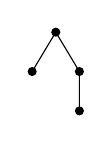
\begin{tikzpicture}[baseline]
\foreach \x/\y/\p in {0/.5/o, -.3/0/a1, .3/0/a2, .3/-.5/b}{
    \coordinate (\p) at (\x,\y);
    \filldraw (\p) circle (0.05);
}
\draw (a1)--(o)--(a2)--(b);
\end{tikzpicture}
\right)=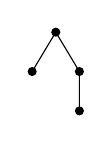
\begin{tikzpicture}[baseline]
\foreach \x/\y/\p in {0/.5/o, -.3/0/a1, .3/0/a2, .3/-.5/b}{
    \coordinate (\p) at (\x,\y);
    \filldraw (\p) circle (0.05);
}
\draw (a1)--(o)--(a2)--(b);
\end{tikzpicture}\otimes1+1\otimes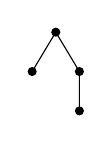
\begin{tikzpicture}[baseline]
\foreach \x/\y/\p in {0/.5/o, -.3/0/a1, .3/0/a2, .3/-.5/b}{
    \coordinate (\p) at (\x,\y);
    \filldraw (\p) circle (0.05);
}
\draw (a1)--(o)--(a2)--(b);
\end{tikzpicture}+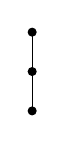
\begin{tikzpicture}[baseline]
\foreach \x/\y/\p in {0/.5/o, 0/0/a, 0/-.5/b}{
    \coordinate (\p) at (\x,\y);
    \filldraw (\p) circle (0.05);
}
\draw (o)--(a)--(b);
\end{tikzpicture}\otimes\begin{tikzpicture}
\filldraw (0,0) circle (0.05);
\end{tikzpicture}+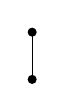
\begin{tikzpicture}[baseline]
\foreach \x/\y/\p in {0/.3/o, 0/-.3/a}{
    \coordinate (\p) at (\x,\y);
    \filldraw (\p) circle (0.05);
}
\draw (o)--(a);
\end{tikzpicture}\otimes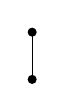
\begin{tikzpicture}[baseline]
\foreach \x/\y/\p in {0/.3/o, 0/-.3/a}{
    \coordinate (\p) at (\x,\y);
    \filldraw (\p) circle (0.05);
}
\draw (o)--(a);
\end{tikzpicture}+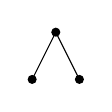
\begin{tikzpicture}[baseline]
\foreach \x/\y/\p in {0/.3/o, -.3/-.3/a1, .3/-.3/a2}{
    \coordinate (\p) at (\x,\y);
    \filldraw (\p) circle (0.05);
}
\draw (a1)--(o)--(a2);
\end{tikzpicture}\otimes\begin{tikzpicture}
\filldraw (0,0) circle (0.05);
\end{tikzpicture}+\begin{tikzpicture}
\filldraw (0,0) circle (0.05);
\end{tikzpicture}\otimes\begin{tikzpicture}
\filldraw (0,0) circle (0.05);
\end{tikzpicture}\;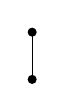
\begin{tikzpicture}[baseline]
\foreach \x/\y/\p in {0/.3/o, 0/-.3/a}{
    \coordinate (\p) at (\x,\y);
    \filldraw (\p) circle (0.05);
}
\draw (o)--(a);
\end{tikzpicture}+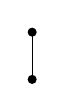
\begin{tikzpicture}[baseline]
\foreach \x/\y/\p in {0/.3/o, 0/-.3/a}{
    \coordinate (\p) at (\x,\y);
    \filldraw (\p) circle (0.05);
}
\draw (o)--(a);
\end{tikzpicture}\otimes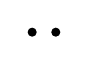
\begin{tikzpicture}
\filldraw (0,0) circle (0.05);
\filldraw (.3,0) circle (0.05);
\end{tikzpicture}
\]
\end{example}

\begin{definition}(see~\cite{Goncharov_GaloisSymmetriesOfFundamentalGroupoidsAndNoncommutativeGeometry}, section 4)
Suppose $S$ is a set. An $S$-decoration of a rooted plane trivalent tree $T$ with $n+1$ leaves is a tuple $(a_0;a_1,\cdots,a_n;a_{n+1})\in S^{n+2}$. See Figure~\ref{fig: decorated trees} for an illustration.
\begin{figure}
\centering
\begin{tikzpicture}
\draw (-1,0)--(7,0);
\foreach \x/\y/\p in {0/0/a0, 1/0/a1, 2/0/a2, 3/0/a3, 4/0/a4, 5/0/a5, 6/0/a6, .5/1/y1, 2.5/1/y2, 4.5/1/y3, 1.5/2/x1, 5/2/x2, 3/3/r}{
    \coordinate (\p) at (\x,\y);
    \filldraw (\p) circle (0.05);
}
\draw (a0)--(y1)--(x1)--(r)--(x2)--(a6);
\draw (r)--($(r)+(0,1)$);
\foreach \p/\q in {y1/a1, x1/y2, y2/a2, y2/a3, x2/y3, y3/a4, y3/a5}{
    \draw (\p)--(\q);
}
\foreach \x/\labeltext in {-.5/{$a_0$},.5/{$a_1$},4.5/{$a_n$},5.5/{$a_{n+1}$}}{
\node at (\x,0)[below] {\labeltext};
}
\end{tikzpicture}
\caption{Decoration on a rooted plane trivalent tree}
\label{fig: decorated trees}
\end{figure}
\end{definition}

We could think of a rooted trivalent plane tree growing down from the root (root is the only node that has one distinguished leg), and all leaves lie on an imaginary line which has been divided by leaves into $n+2$ parts labeled as $a_0,a_1,\cdots,a_n,a_{n+1}$ in order.

\begin{remark}
A subtree of $T$ also has a decoration from the decoration of $T$, which is just a contiguous subsequence $(a_i;a_{i+1},\cdots,a_{j-1};a_j)$.
\end{remark}

\begin{theorem}\label{thm: Connes-Kreimer coproduct}(see~\cite{Goncharov_GaloisSymmetriesOfFundamentalGroupoidsAndNoncommutativeGeometry}, section 4)
The free algebra $\mathcal T(S)$ generated by $S$-decorated rooted plane trivalent trees again forms a graded Hopf algebra with Connes-Kreimer's coproduct on trees.
\end{theorem}

\begin{theorem}\label{thm: embedding of I(S) -> T(S)}(see~\cite{Goncharov_GaloisSymmetriesOfFundamentalGroupoidsAndNoncommutativeGeometry}, section 4)
Suppose $S$ is a set, and let $\widetilde{\mathcal I}(S)$ be the free graded algebra generated by $I(a_0;a_1,\cdots,a_n;a_{n+1}),a_i\in S$ in weight $n\geq1$. Then it is a graded Hopf algebra with coproduct
\begin{multline}\label{eq: Coproduct for iterated integrals}
\Delta I(a_0;a_1,\cdots;a_n;a_{n+1})=\\
\sum_{0=i_0<i_1<\cdots<i_k<i_{k+1}=n+1}I(a_{i_0};a_{i_1},\cdots,a_{i_k};a_{i_{k+1}})\otimes\prod_{p=0}^kI(a_{i_p};a_{i_p+1},\cdots,a_{i_{p+1}-1};a_{i_{p+1}})
\end{multline}
Here we assume $I(a;b)=1$ for all $a,b$.
\end{theorem}

\begin{proof}
There is an embedding of $\widetilde{\mathcal I}(S)$ into $\mathcal T(S)$ that maps $I(a_0;a_1,\cdots,a_n;a_{n+1})$ to the sum of rooted plane trivalent trees with decoration $(a_0;a_1,\cdots,a_n;a_{n+1})$.
\end{proof}

\begin{example}
\begin{align*}
\Delta I(a_0;a_1,a_2,a_3;a_4)&=1\otimes I(a_0;a_1,a_2,a_3;a_4)+I(a_0;a_1;a_4)\otimes I(a_1;a_2,a_3;a_4)\\
&+I(a_0;a_2;a_4)\otimes I(a_0;a_1;a_2)I(a_2;a_3;a_4)+I(a_0;a_3;a_4)\otimes I(a_0;a_1,a_2;a_3)\\
&+I(a_0;a_1,a_2;a_4)\otimes I(a_2;a_3;a_4)+I(a_0;a_1,a_3;a_4)\otimes I(a_1;a_2;a_3)\\
&+I(a_0;a_2,a_3;a_4)\otimes I(a_0;a_1;a_2)+I(a_0;a_1,a_2,a_3;a_4)\otimes1
\end{align*}
\end{example}

Since an iterated integral evaluates to zero if its integration path is the trivial constant path at a point, we sometimes wish to get rid of such elements in $\widetilde I(S)$.

\begin{definition}
Elements like $I(a;\cdots;a)$ that start and end with the same element are called \textit{degenerate}. Define $\mathcal I(S)$ to be $\widetilde{\mathcal I}(S)$ modulo degenerates.
\end{definition}

\begin{proposition}
$\mathcal I(S)$ is a graded Hopf algebra with a coproduct induced from Theorem~\ref{thm: embedding of I(S) -> T(S)}.
\end{proposition}

\begin{proof}
It is not hard to see that the ideal generated by degenerates is a homogeneous Hopf ideal. So the quotient algebra $\mathcal I(S)$ of $\widetilde{\mathcal I}(S)$ is again a graded Hopf algebra according to Proposition~\ref{prop: quotient Hopf algebra}.
\end{proof}

\subsection{Symbols of multiple polylogarithms}\label{sec: symbols of Gangl}

Herbert Gangl, Goncharov et al. explored the symbols of multiple polylogarithms (see~\cite{Gangl_FromPolygonsAndSymbolsToPolylogarithmicFunctions}).

\begin{definition}
The symbol of a hyperlogarithm $I(a_0;\cdots;a_{n+1})$ is its image under $\Delta_{1,\cdots,1}$
\end{definition}

\begin{example}
The symbol of $I(a_0;a_1,a_2,a_3;a_4)$ is
\begin{multline}
I(a_0;a_1;a_4)\otimes I(a_1;a_2;a_4)\otimes I(a_2;a_3;a_4)+I(a_0;a_1;a_4)\otimes I(a_1;a_3;a_4)\otimes I(a_1;a_2;a_3)\\
+I(a_0;a_2;a_4)\otimes I(a_0;a_1;a_2)\otimes I(a_2;a_3;a_4)+I(a_0;a_2;a_4)\otimes I(a_2;a_3;a_4)\otimes I(a_0;a_1;a_2)\\
+I(a_0;a_3;a_4)\otimes I(a_0;a_1;a_3)\otimes I(a_1;a_2;a_3)+I(a_0;a_3;a_4)\otimes I(a_0;a_2;a_3)\otimes I(a_0;a_1;a_2)
\end{multline}
\end{example}

\begin{example}\label{ex: symbol of Li_{2,1}(x_1,x_2)}
Similarly, we can compute the symbol of multiple polylogarithm $\Li_{2,1}(x_1,x_2)$, the previous example becomes
\begin{multline}
\Delta_{1,\cdots,1}(\Li_{2,1}(x_1,x_2))=\Delta_{1,\cdots,1}\left(I\left(0;\frac{1}{x_1x_2},0,\frac{1}{x_2};1\right)\right)=\\
\Li_1\left(x_2\right)\otimes \Li_1\left(x_1\right)\otimes \log\left(x_1\right)-\Li_1\left(x_1 x_2\right)\otimes \log \left(x_1\right)\otimes \log
   \left(x_1\right)\\
+\Li_1\left(x_1 x_2\right)\otimes \log \left(x_1 x_2\right)\otimes \Li_1\left(x_2\right)-\Li_1\left(x_1 x_2\right)\otimes
   \Li_1\left(x_1\right)\otimes \log \left(x_1\right)\\
+\Li_1\left(x_1 x_2\right)\otimes \Li_1\left(x_2\right)\otimes \log \left(x_1\right)
\end{multline}
\end{example}

\subsection{Monodromies of multiple polylogarithms}\label{sec: Zhao's calc on monodromy of multiple logarithms}

In~\cite{Zhao_MultipleZetaFunctionsMultiplePolylogarithmsAndTheirSpecialValues}, Zhao described a variation of mixed Hodge structures encoded by multiple polylogarithms and computed the monodromies for multiple logarithms. Firstly, let us describe the fundamental group of $S_d(\mathbb C)$.

\begin{theorem}[\cite{ZackThesis}]
$\pi_1(S_d(\mathbb C))$ is the free group generated by loops around the divisors
\[
\{x_r=0\}\text{ and }\{x_j\cdots x_k=1\}
\]
More specifically, it is torsion free of rank $2d+\binom{d}{2}$, generated by $\nu_r$, $1\leq r\leq d$ and $\nu_{jk}$, $1\leq j\leq k\leq d$, where $\nu_r$ is the positive loop around the divisor $x_r=0$, i.e.
\[
\int_{\nu_r}d\log(x_s)=2\pi i\delta_{rs},\quad\int_{\nu_i}d\log(1-x_j\cdots x_k)=0
\]
and $\nu_{j,k}$ is the positive loop around the divisor $x_j\cdots x_k=1$, i.e.
\[
\int_{\nu_{j,k}}d\log(x_s)=0,\quad\int_{\nu_{j,k}}d\log(1-x_p\cdots x_q)=2\pi i\delta_{jp}\delta_{kq}
\]
Here $\delta$ is the Kronecker delta.
\end{theorem}

Zhao also gives concrete choices for $\nu_r,\nu_{j,k}$. For example, $\nu_r$ could be a loop in some plane $\{x_s=a_s\neq 0,\forall s\neq r\}$ such that
\[
\oint_{\nu_r}\dfrac{dz}{z}=2\pi i,\quad\oint_{\nu_{j,k}}\dfrac{dz}{z-1}=0
\]
and $\nu_{j,k}$ could be a loop in some plane $\{x_s=a_s\neq 0,\forall s\neq r\}$ where any products of $a_s$ does not equal to 1, and $\nu_{j,k}$ satisfies
\[
\oint_{\nu_r}\dfrac{dz}{z}=0,\quad\oint_{\nu_{j,k}}\dfrac{dz}{z-1}=2\pi i
\]

Zhao's strategy is to convert these iterated integrals on $\mathbb C$ into iterated integrals on $S_d(\mathbb C)$, and then use this to compute the monodromies of multiple logarithms.

\begin{theorem}
Multiple polylogarithms can be expressed as iterated integrals of logarithmic differential forms over $S_d(\mathbb C)$.
\end{theorem}

\begin{example}
\begin{multline}
\Li_{1,1}(x_1,x_2)=\int_{(0,0)}^{(1,1)}\frac{dx_2}{1-x_2}\frac{dx_1}{1-x_1}+\frac{d(x_1x_2)}{1-x_1x_2}\left(\frac{dx_2}{1-x_2}+\frac{dx_1}{x_1(x_1-1)}\right)
\end{multline}
\end{example}

Let's denote the monodromy operator as $\mathcal M_{\nu_i}$ and $\mathcal M_{\nu_{j,k}}$. Zhao has the following theorem describing the monodromy of multiple logarithms - multiple polylogarithms $\Li_{n_1,\cdots,n_d}$ with $\mathbf n=(n_1,\cdots,n_d)=(1,\cdots,1)$. In Chapter 5,  we will generalize the theorem to arbitrary $\mathbf n$.

\begin{theorem}\label{thm: Zhao's monodromy thm}
\begin{equation}
(\mathcal M_{\nu_i}-\id)\Li_{1,\cdots,1}(x_1,\cdots,x_d)=0,\quad 1\leq i\leq d
\end{equation}
\begin{equation}
(\mathcal M_{\nu_{j,k}}-\id)\Li_{1,\cdots,1}(x_1,\cdots,x_d)=0,\quad\forall 1\leq j<k<d
\end{equation}
\begin{equation}
(\mathcal M_{\nu_{j,j}}-\id)\Li_{1,\cdots,1}(x_1,\cdots,x_d)=0,\quad\forall 1\leq j<d
\end{equation}
\begin{equation}
(\mathcal M_{\nu_{d,d}}-\id)\Li_{1,\cdots,1}(x_1,\cdots,x_d)=2\pi i\Li_{1,\cdots,1}(x_1,\cdots,x_{d-1})
\end{equation}
\begin{multline}
(\mathcal M_{\nu_{j,d}}-\id)\Li_{1,\cdots,1}(x_1,\cdots,x_d)=2\pi i\Li_{1,\cdots,1}(x_1,\cdots,x_{j-1})\\
\Li_{1,\cdots,1}\left(\frac{1-x_jx_{j+1}}{1-x_j},\cdots,\frac{1-x_j\cdots x_d}{1-x_j\cdots x_{d-1}}\right),\quad \forall 1\leq j<d
\end{multline}
\end{theorem}

\section{Variation of mixed Hodge structures}

Multiple polylogarithms naturally define variations of mixed Hodge structures. These mixed Hodge structures are described by filtrations on the flat sections of a vector bundle, so first we need to review connections on vector bundles and how they are related to local systems with monodromies.

\subsection{Connection on vector bundles}

\begin{definition}
Suppose $B$ is a complex manifold and $E\to B$ is a vector bundle. The $E$ valued $k$-forms are defined to be
\[\Omega^k(E)=\Gamma\left(\textstyle\bigwedge^kT^*B\otimes E\right)=\Omega^k(B)\otimes\Gamma(E)\]
a \textit{vector bundle(Koszul) connection} is
\[\nabla:\Omega^0(E)\to\Omega^1(E)=T^*B\otimes\Gamma(E)\]
satisfying the Leibniz rule
\begin{equation}\label{Koszul connection}
\nabla (f\otimes s)=df\otimes s+f\wedge\nabla s
\end{equation}
A vector field $X\in TB$ defines the covariant derivative $\nabla_X:\Gamma(E)\to\Gamma(E)$ along $X$, which by~\eqref{Koszul connection} uniquely extends to a exterior covariant derivative $\nabla:\Omega^k(E)\to\Omega^{k+1}(E)$ through
\[
\nabla (\omega\otimes s)=d\omega\otimes s+(-1)^{|\omega|}\omega\wedge\nabla s
\]
\end{definition}

\begin{definition}[Connection form] \hfill\\
Over a local trivialization, suppose $s=\sum_i s_i\otimes e_i$, $\nabla e_i=\sum_j\omega_{ji}\otimes e_j$, then
\[
\nabla s=\sum_ids_i\otimes e_i+\sum_is_i\wedge\left(\sum_j\omega_{ji}\otimes e_j\right)=\sum_i\left(ds_i+\sum_j\omega_{ij}\wedge s_j\right)\otimes e_i
\]
In short, we have $\nabla s=ds+\omega\wedge s$, where $\omega=(\omega_{ij})$ is known as the \textit{connection form}.
% Suppose $\theta^i$ is a dual basis of $e_i$, i.e. $\theta^i(e_j)=\delta_{ij}$, since $\nabla_{e_i}e_j=\sum_k\Gamma^k_{ij}e_k$, we should have $\omega_{kj}=\sum_i\Gamma^k_{ij}\theta^i$
\end{definition}

\begin{definition}[Curvature]\label{def: curvature}
The curvature tensor is defined as
\[\nabla^2:\Omega^0(E)\to\Omega^2(E)\]
Over a local trivialization, $\nabla^2s=\nabla(ds+\omega\wedge s)=(d\omega+\omega\wedge\omega)\wedge s$, thus $d\omega+\omega\wedge\omega$ is called the \textit{curvature form}. A connection is \textit{flat(completely integrable)} if its curvature is zero.
\end{definition}

\begin{proposition}\label{prop: conjugate connection}
If $\phi$ is an automorphism of $E\to B$, the conjugate $\nabla^\phi=\phi^{-1}\circ\nabla\circ\phi$ is again a connection. Furthermore, $\nabla^\phi$ is flat if $\nabla$ is flat.
\end{proposition}

\begin{proof}
\begin{align*}
\nabla^\phi(f\otimes s)&=\phi^{-1}\circ\nabla(f\otimes\phi s)=\phi^{-1}(df\otimes \phi s+f\wedge \nabla(\phi s))=df\otimes s+f\wedge\nabla^\phi s
\end{align*}
Over a local trivialization, $\phi s=As$. We then have
\begin{align*}
A^{-1}(\nabla(As))&=A^{-1}(d(As)+\omega\wedge As)=A^{-1}(dAs+Ads+\omega\wedge As)\\
&=ds+(A^{-1}dA+A^{-1}\omega A)s
\end{align*}
Hence the connection form for $\nabla^\phi$ is $A^{-1}dA+A^{-1}\omega A$. If $d\omega+\omega\wedge\omega=0$, then
\[
d(A^{-1}dA+A^{-1}\omega A)+(A^{-1}dA+A^{-1}\omega A)\wedge(A^{-1}dA+A^{-1}\omega A)=0
\]
Hence, $\nabla^\phi$ is a flat connection.
\end{proof}

We can rephrase vector bundles as locally free sheaves.

\begin{definition}
Suppose $B$ is a complex manifold and $E\to B$ is a vector bundle. The sheaf of sections of $E$ is a locally free sheaf $\mathcal E$, and a connection $\nabla$ on $E$ can be naturally generalized as a connection on $\mathcal E$, via $\nabla:\Omega_B^k\otimes_{\mathcal O_B}\mathcal E\to\Omega_B^{k+1}\otimes_{\mathcal O_B}\mathcal E$
\[
\nabla (\omega\otimes s)=d\omega\otimes s+(-1)^{|\omega|}\omega\wedge\nabla s
\]
\end{definition}

Note that locally $\Gamma(\Omega^k_U\otimes_{\mathcal O_U}\mathcal E_U)\cong\Omega^k(E|_U)$. So we can define connection form $\omega=(\omega_{ij})$ as well.

\begin{theorem}[Riemann-Hilbert Correspondence]
Suppose $B$ is a complex manifold. The category of locally constant sheaves of vector spaces is equivalent to the category of locally free sheaves with flat connections.
\end{theorem}

\begin{proof}
Suppose $\mathbb V$ is a locally constant sheaf, then $\mathcal V=\mathcal O_B\otimes_{\underline{\mathbb Z}}\mathbb V$ is a locally free sheaf, and $\nabla(f\otimes v)=df\otimes v$ defines a flat connection. On the other hand, suppose $\mathcal E$ is a locally free sheaf with a flat connection $\nabla$ with connection form $\omega$. Then the sheaf of flat sections forms a locally constant sheaf. If we take the boundary $\partial R$ of a simple region $R$, and suppose $f$ is a flat section so that $df+\omega\wedge f=0$ locally, then
\[
\int_{\partial R}df=\int_{R}d^2f
\]
But locally we have
\begin{align*}
d^2f&=d(-\omega\wedge f)\\
&=\omega\wedge df-d\omega\wedge f\\
&=-\omega\wedge\omega\wedge f+\omega\wedge\omega\wedge f\\
&=0
\end{align*}
Therefore $f$ can be well defined on the universal cover of $B$, thus giving a locally constant sheaf.
\end{proof}

Deligne~\cite{Deligne_EquationsDifferentiellesAPointsSinguliersReguliers} extended this result, a generalization necessary for constructing the variation of mixed Hodge structures in Chapter 4.

\begin{theorem}\label{thm: Deligne's thm flat connection <=> local system}
Suppose $\overline X$ is a projective variety with $X\subseteq\overline X$ and $D=\overline X-X$ is a simple normal crossing. The category of locally constant sheaves of vector spaces is equivalent to locally free sheaves with connections.
\end{theorem}

\subsection{Hodge structures and variations of mixed Hodge structures}

Suppose $H$ is a finitely generated abelian group, and denote $H_R=H\otimes R$ for any $\mathbb Z$-module $R$.

\begin{definition}
We say $H$ has a pure Hodge structure of weight $n$ if there is a finite decreasing Hodge filtration $F^\bullet$ of $H_{\mathbb C}$ by subspaces $\{F^pH_{\mathbb C}\}_{p\in\mathbb Z}$ such that
\[
H_{\mathbb C}=F^pH_{\mathbb C}\oplus\overline{F^{n+1-p}H_{\mathbb C}}
\]
If we denote $H^{p,n-p}=F^pH_{\mathbb C}\cap \overline{F^{n-p}H_{\mathbb C}}$, we then have the Hodge decomposition
\[
H_{\mathbb C}=\bigoplus_{p+q=n}H^{p,q}
\]
\end{definition}

\begin{definition}
Suppose $H$ is a finitely generated abelian group. We say it has a mixed Hodge structure if there is a finite decreasing Hodge filtration $F^\bullet$ of $H_{\mathbb C}$ by subspaces $\{F^pH_{\mathbb C}\}_{p\in\mathbb Z}$ and an increasing weight filtration $W^\bullet$ of $H_{\mathbb Q}$ by subspaces $\{W_kH_{\mathbb Q}\}_{k\in\mathbb Z}$ such that the graded piece $gr^W_kH_{\mathbb Q}$ is a pure Hodge structure of weight $k$ with Hodge filtration given by
\[
F^p(gr^W_kH_{\mathbb Q})_{\mathbb C}=\frac{F^pH_{\mathbb C}\cap (W_{k+1}H_{\mathbb Q})_{\mathbb C}+(W_kH_{\mathbb Q})_{\mathbb C}}{(W_kH_{\mathbb Q})_{\mathbb C}}
\]
\end{definition}

% \begin{definition}
% A polarization $Q$ of $H$ is a non-degenerate bilinear form such that
% \[
% \begin{cases}
% Q(\phi,\psi)=(-1)^nQ(\psi,\phi),\forall\phi,\psi\in H_{\mathbb C}\\
% Q(\phi,\psi)=0,\forall\phi\in H^{p,q}_{\mathbb C},\psi\in H^{p',q'}_{\mathbb C},p\neq q' \\
% i^{p-q}Q(\phi,\overline\phi)>0,\forall\phi\in H^{p,q}_{\mathbb C},\phi\neq0
% \end{cases}
% \]
% Or in terms of the hodge filtration
% \[
% \begin{cases}
% Q(F^pH_{\mathbb C},F^{p+1}H_{\mathbb C})=0\\
% Q(C\phi,\overline\phi)>0,\forall\phi\in H_{\mathbb C},\phi\neq0
% \end{cases}
% \]
% Here $C$ is the Weil operator which is the direct sum of $i^{p-q}$ on $H^{p,q}_{\mathbb C}$
% \end{definition}

% If every fiber of a vector bundle has a mixed Hodge structures that varies holomorphically, we call it a variation of mixed Hodge structures.

Let $B$ be a complex manifold and $\mathbb V$ a locally constant sheaf of finitely generated abelian groups, then $\mathbb V_{\mathbb Q}=\mathbb V\otimes_{\underline{\mathbb Z}}\underline{\mathbb Q}$, $\mathbb V_{\mathbb C}=\mathbb V\otimes_{\underline{\mathbb Z}}\underline{\mathbb C}$ are locally constant sheaves of vector spaces, and $\mathcal V=\mathbb V\otimes_{\underline{\mathbb Z}}\mathcal O_B$ is a locally free sheaf.

\begin{definition}
A \textit{variation of pure Hodge structures} of weight $n$ is a decreasing filtration $F^\bullet$ of $\mathcal V$ by subsheaves $\{F^p\mathcal V\}$ such that each fiber $\mathbb V_{b}$ is a pure Hodge structure of weight $n$ with Hodge filtration $\{F^p\mathbb V_{\mathbb C,b}\}$ which satisfies Griffith transversality: $\nabla F^p\mathcal V\subseteq F^{p-1}\mathcal V\otimes\Omega^1_B$.
\end{definition}

\begin{definition}
A \textit{variation of mixed Hodge structures} consists of a decreasing filtration $F^\bullet$ of $\mathbb V$ by holomorphic subsheaves $\{F^p\mathcal V\}$, and a weight filtration $W_\bullet$ of $\mathbb V_{\mathbb Q}$ by subsheaves $\{W_k\mathbb V_{\mathbb Q}\}$ such that each fiber $\mathbb V_b$ is a mixed Hodge structure with Hodge filtration $F^p\mathbb V_{\mathbb C,b}$ and weight filtration $W_k\mathbb V_{\mathbb Q,b}$, again satisfying the Griffith transversality $\nabla F^p\mathcal V\subseteq F^{p-1}\mathcal V\otimes\Omega^1_B$.
\end{definition}


\section{Relation between iterated integrals and motivic cohomology}

The following discussion can be found in~\cite{Goncharov_GaloisSymmetriesOfFundamentalGroupoidsAndNoncommutativeGeometry}.

Suppose $\mathcal M(F)$ is the category of mixed Tate motives over a number field $F$ with pure Tate motives $\mathbb Q(n)$. The $i$-th motivic cohomology group $H^i_{\mathcal M}(F,\mathbb Q(n))$ is defined as $i$-th Ext group $\Ext^i_{\mathcal M(F)}(\mathbb Q(0),\mathbb Q(n))$. Since $\mathcal M(F)$ is a Tannakian category, $\mathcal M(F)$ is equivalent to the category of finite-dimension modules over $\Aut^{\otimes}\Psi$, where
\[
\Psi:\mathcal M(F)\to\operatorname{Vect}_{\mathbb Q},\quad M\mapsto\textstyle\bigoplus\limits_n\Hom(\mathbb Q(n),\Gr^W_{2n}M)
\]
is the fiber functor, and $\Aut^{\otimes}\Phi$ is the group scheme of automorphisms of $\Phi$ respecting the tensor product.

$\Aut^{\otimes}\Psi$ is the semidirect product of the multiplicative group scheme $\mathbb G_m$ and a pro-unipotent group scheme $U(F)$, denote $L(F)$ as the Lie algebra of $U(F)$, $L(F)$ is graded due to the action of $\mathbb G_m$. Then $\mathcal U(F)=\End(\Psi)$ is isomorphic to the universal enveloping algebra of $L(F)$. Suppose $\mathcal H(F)$ is the dual of $\mathcal U(F)$, then $\mathcal H(F)$ can be identified with the graded Hopf algebra of regular functions on $U(F)$, and $\mathcal L(F)=\dfrac{\mathcal H_{>0}(F)}{\mathcal H_{>0}(F)\cdot\mathcal H_{>0}(F)}$ is a graded Lie coalgebra, the cotangent space of $U(F)$ which is dual of $L(F)=\Lie(U(F))$.

Goncharov constructed a Hopf algebra $\mathcal A(F)$ (see~\cite{Goncharov_GaloisSymmetriesOfFundamentalGroupoidsAndNoncommutativeGeometry}) as the set of equivalences classes of framed mixed Tate motives $I^{\mathcal M}(a_0;a_1,\cdots,a_n;a_{n+1})$, with the coproduct similar to the coproduct~\eqref{eq: Coproduct for iterated integrals} for iterated integrals, and showed that $\mathcal A(F)$ and $\mathcal H(F)$ are canonically isomorphic. He then considered its realizations in various categories, the benefit of this is that in each case we get a coproduct and Hopf algebra structure for free.